% ==============================================================================
% thesis.tex
% Example file for tumthesis.csl
% Michael Ritter, 2012
% Licence:
% This work may be distributed and/or modified under the
% conditions of the LaTeX Project Public License, either version 1.3
% of this license or (at your option) any later version.
% The latest version of this license is in
% http://www.latex-project.org/lppl.txt
% and version 1.3 or later is part of all distributions of LaTeX
% version 2005/12/01 or later.
% ==============================================================================
\documentclass[]{tumthesis}

\usepackage[T1]{fontenc}
\usepackage{lmodern}
\usepackage[utf8]{inputenc}

\usepackage{color}
\usepackage{tocbibind}

\usepackage{listings}
% JavaScript
\lstdefinelanguage{JavaScript}{
  morekeywords={typeof, new, true, false, catch, function, return, null, catch, switch, var, if, in, while, do, else, case, break},
  morecomment=[s]{/*}{*/},
  morecomment=[l]//,
  morestring=[b]",
  morestring=[b]'
}

% ------------------------------------------------------------------------------
%FixMe-Status: final (no FixMe comments) or draft (comments visible)
%\fxsetup{draft}
\fxsetup{final}
% ------------------------------------------------------------------------------

% ------------------------------------------------------------------------------
%  Language selection for metadata and main text (can be changed at any point in
%  the main text.
\selectlanguage{ngerman}
%\selectlanguage{english}
% ------------------------------------------------------------------------------

% ------------------------------------------------------------------------------
% Data for the bibliography
\addbibresource{thesis.bib}
% ------------------------------------------------------------------------------

% ------------------------------------------------------------------------------
% Further packages and TikZ libraries can be incorporated here.
\usetikzlibrary{arrows}
% ------------------------------------------------------------------------------

% ------------------------------------------------------------------------------
% Using the include-command: The content of the work will be incorporated using
% the include-command. So that you can test things out without always needing
% the full thesis, you can define here which sections will be incorporated and
% which will not. Of course, for the final version you should be sure to
% incorporate everything.
%\includeonly{%
%titlepage,%
%declaration,%
%abstract,%
%introduction,%
% include own sections here (rule of thumb: one file per chapter)
%conclusion,%
%appendix%
%}%
% ------------------------------------------------------------------------------

\def\defTitle{Visualisierung von Flussalgorithmen}
\def\defSubject{
\texttt{Ford-Fulkerson} Algorithmus \\
\textit{zur Lösung des Maximum Flow Problems} \\
\texttt{Cycle Canceling} Algorithmus \\
\textit{zur Lösung des Minimum-Cost Flow Problems}}

% ------------------------------------------------------------------------------
% PDF-Metadaten
\hypersetup{
 pdfauthor={Quirin Fischer},
 pdftitle={\defTitle},
 pdfsubject={\defSubject},
 pdfkeywords={IDP},
 %colorlinks=true, %coloured links (for the PDF version)
 colorlinks=false, % no coloured links (for the print version)
 bookmarksnumbered=true,     
 bookmarksopen=true,         
 bookmarksopenlevel=1,
 pdfstartview=Fit,           
 %pdfpagemode=UseOutlines,    % this is the option you were lookin for
 pdfpagelayout=TwoPageRight,
    pdfborder={0 0 0},
}
% ------------------------------------------------------------------------------

% ------------------------------------------------------------------------------
% Data for the title page and declaration
\author{Quirin Fischer}
\title{\defTitle}
\subtitle{\defSubject}
\faculty{Fakultät für Mathematik}
\institute{Lehrstuhl für Angewandte Geometrie und Diskrete Mathematik}
%\subject{master}
%\subject{bachelor}
%\subject{diploma}
%\subject{project}
%\subject{seminar}
\subject{idp}
\subject{Interdisziplinäres Projekt (IDP)}
\professor{Prof. Dr. Peter Gritzmann} %Themensteller
\advisor{M.Sc. Wolfgang F. Riedl} %Betreuer
\date{30.09.2016} %Submission Date
\place{München} %Place where document is signed
% ------------------------------------------------------------------------------

% ==============================================================================
% Main part of the document
% ==============================================================================
\makeindex[title=Index,options=-s myindex]
\begin{document}
\pagestyle{empty}
\frontmatter%
\selectlanguage{ngerman}
%\selectlanguage{english}
\maketitlepage%
\makedeclaration%


\cleardoublepage
\addcontentsline{toc}{chapter}{Abstract / Zusammenfassung}
\selectlanguage{english}
\section*{Abstract}

This interdisciplinary project encompasses the development of interactive applications to visualise two flow algorithms: The Ford-Fulkerson algorithm for solving the maximum-flow problem, and the cycle canceling algorithm for solving the minimum-cost flow problem. This report presents the algorithms, describes the layout of the applications, and explains the technical realisation.

The aim of the applications is to facilitate the comprehension of the algorithms by allowing the step-by-step execution on any desired instance of the problem, displaying the computational phases transparently, and graphically visualising the data structures.

The implementation is done as an application for web browsers by using an existing framework which uses modern web standards like HTML5, SVG, CSS, Javascript and D3.js. In particular, multiple important components of the implementation and their interactions are described in order to give a clear overview of the code base. 


\selectlanguage{ngerman}
\section*{Zusammenfassung}

Dieses interdisziplinäre Projekt umfasst die Entwicklung von interaktiven Anwendungen für die Visualisierung zweier Flussalgorithmen: Des Ford-Fulkerson Algorithmus zur Lösung des Maximum-Flow Problems, und des Cycle-Canceling Algorithmus zur Lösung des Minimum-Cost Flow Problems. Dieser Bericht stellt die Algorithmen vor, beschreibt den Aufbau der Applikationen, und erläutert die technische Umsetzung. 

Das Ziel der Applikationen ist das Verständnis der Algorithmen zu erleichtern, indem eine schrittweise Ausführung an beliebigen Instanzen des Problems ermöglicht, die Berechnungsschritte sichtbar gemacht und Datenstrukturen anschaulich visualisiert werden.

Die Implementierung erfolgt als Webapplikation für den Browser mithilfe eines bestehenden Frameworks, das moderne Webstandards wie HTML5, SVG, CSS, Javascript und D3.js verwendet. Insbesondere werden verschiedene wichtigen Komponenten der Implementierung und deren Zusammenspiel behandelt, um einen klaren Überblick über den Code zu geben.

\selectlanguage{ngerman}


\tableofcontents%

\mainmatter%
\pagestyle{headings}

%% ==============================
\addcontentsline{toc}{chapter}{Einleitung}
\chapter*{Einleitung}
%% ==============================

Die Graphentheorie ist eine Teilgebiet der (diskreten) Mathematik mit einigen herausstellenden Merkmalen: Sie ist sehr anwendungsbezogen, da viele praktische Entscheidungsprobleme mithilfe von Graphen modelliert werde können. Sie hat weiterhin eine sehr enge Verbindung zur Algorithmik, wobei sowohl algorithmische Probleme mit bestimmten Graphen zusammenhängen, als auch Probleme der Graphentheorie mithilfe von Algorithmen gelöst werden, und daraus folgend auch zur Informatik. Aufrund ihrer Anschaulichkeit und der Nützlichkeit der Konzepte ist die Graphentheorie einer der ersten Bereiche der Mathematik mit dem Studenten mathematischer, informatischer oder technischer Fachrichtungen in Berührung kommen.

Eine besonders charakteristischer Teil hierbei ist die Beschäftigung mit verschiedenen Graphalgorithmen. Das Verständnis der Abläufe, der Eigenschaften und Strukture die der einzelne Algorithmus ausnutzt, und den entsprechenden Eigenschaften der resultierenden Lösungen gibt eine vielseitige Perspektive auf die behandelten Problemstellungen. Eine wichtiges Hilfsmittel für die Einarbeitung in neue Algorithmen sind dabei die ausführliche Durchführung des Algorithmuses auf verschiedenen Beispielen und Betrachtung der Berechnungsschritte. Insbesondere die Visualisierung des Graphen mit verschiedenen Annotationen ist vielmals hilfreich um ein Gefühl für die Vorgänge zu bekommen.

Eine Klasse von Graphalgorithmen mit vielseitigen Anwendungen sind Flussprobleme. Abgeleitet von praktischen Fragestellungen zum Transport in verschiedenartigen Netzwerken, man denke an Rohrnetze, Straßennetze oder Datennetzwerke, behandeln sie Optimierungsprobleme wie eine Menge an Ressourcen von einem Start- zu einem Zielknoten gelangen kann. Je nach speziellen Anforderungen wird der Graph, der die Netzwerktopologie modelliert, mit verschiedenen Informationen annotiert. Typischerweise sind dies Kapazitäten (verschiedene Teile des Netzwerkes können nur bestimmte Mengen an Ressource transportieren) oder Kosten (die Benutzung mancher Teile des Netzwerks is anderen vorzuziehen).

Dieses Dokument beschreibt die Entwicklung einer interaktiven Anwendung zur Visualisierung zweier Flussalgorithmen - des Ford-Fulkerson Algorithmus für das Maximum-Flow Problem, und des Cycle Canceling Algorithmus für das Min-Cost Flow Problem. Die Anwendung hat das Ziel das Verständnis der Algorithmen zu erleichtern, indem sie einfach Schritt für Schritt auf verschiedene Instanzen des Problems ausgeführt werden können, mit transparenter Anzeige des Berechnungszustandes und anschaulicher Darstellung der Datenstrukturen. 

Im erste Kapitel werden die zwei behandelten Probleme und Lösungsalgorithmen behandelt. Im zweiten Kapitel wird der Aufbau der Anwendung und ihre verschiedenen Elemente beschrieben. Das dritte Kapitel beschreibt die technische Umsetzung, mit zunächst einem Überblick über die verwendeten Basistechnologien und schließlich einer Behandlung der Implementierung interessanter Komponenten und deren Zusammenspiel.
\chapter{Behandelte Flussalgorithmen}

%Definition von Flussnetzwerken
\section{Flüsse in Netzwerken}

Anschaulich entsprechen Flüsse in Netzwerken der Modellierung von Transportsystemen - Anwendungsfälle sind beispielsweise Wassernetze (wobei Kapazitäten den Rohrdurchmessern entsprechen, und die Menge an geflossenem Wasser dem Fluss), Straßensysteme (Kapazität: Spurbreite, Fluss: beförderte Fahrzeuge) oder Datennetze (Kapazität: Übertragungsgeschwindigkeit, Fluss: übermittelte Datenmenge).

Als Netzwerk bezeichnet man einen gerichteten Graphen $G=\left(V, E\right)$ annotiert mit einer Kapazitätsfunktion für Kanten $u: E \rightarrow \mathbb{R}^+$ (dem \emph{upper limit}), Startknoten $s$ (der \emph{source}) und Zielknoten $t$ (\emph{target}). Insgesamt notiert man folglich ein Netzwerk als 4-Tupel $N = \left(G, u, s, t\right)$. \cite{ wiki:fluesse}

Ein Fluss in einem Netz ist definiert als eine Funktion $f: E \rightarrow \mathbb{R}^+$  (auch \emph{flow}), die für jede Kante des Graphen einen Menge an Fluss bestimmt. Ein gültiger s-t-Fluss  $f$ in einem Netzwerk muss weiterhin zwei Bedingungen erfüllen:

\begin{description}
    \item [Kapazitätskonformität] Der Fluss muss auf allen Kanten unter deren Kapazitätsgrenze liegen:
    \[\forall e \in E :f(e)\leq u(e)\]
    \item [Flusserhalt] Der Fluss ist in allen Knoten abgesehen von $s$ und $t$ Konstant, es gelangt gleich viel Fluss zum Knoten, wie ihn verlässt. Bezeichnet man die Menge an eingehenden Kanten eines Knotens als $\operatorname{\delta^-}(v)\overset{\underset{\mathrm{def}}{}}{=}\{e=(x,v) \in E \mid x \in V \}$ und die Menge an ausgehenden Kanten als $\operatorname{\delta^+}(v)\overset{\underset{\mathrm{def}}{}}{=}\{e=(v,x) \in E \mid x \in V \}$, so entspricht dies der Bedingung 
    \[\forall v\in V \setminus \{s,t\} :\sum_{e\in \operatorname{\delta^-}(v)}f(e)
=\sum_{e \in \operatorname{\delta^+}(v)}f(e)\]
\end{description}

Ein wichtiges Konzept für Flussalgorithmen ist die Konstruktion des zu einem Fluss gehörigen Residualnetzwerkes. Dieses verwendet die gleiche Knotenmenge, enthält allerdings eine neu konstruierte Kantenmenge und andere Kapazitäten. Intuitiv modelliert das Residualnetzwerk welche Änderungen des Flusses möglich sind - es enthält jede Kanten der ursprünglichen Netzwerks, falls zusätzlicher Fluss auf der Kante möglich ist, mit angepasster Kapazität. Für Kanten, die bereits Fluss tragen, werden zusätzlich Rückkanten mit Kapazität entsprechend des Flusses auf der Kante eingefügt, da es möglich wäre, diesen Fluss wieder zurückzuleiten.

\vspace{0.5cm}
\begin{minipage}[t]{0.99\textwidth}
    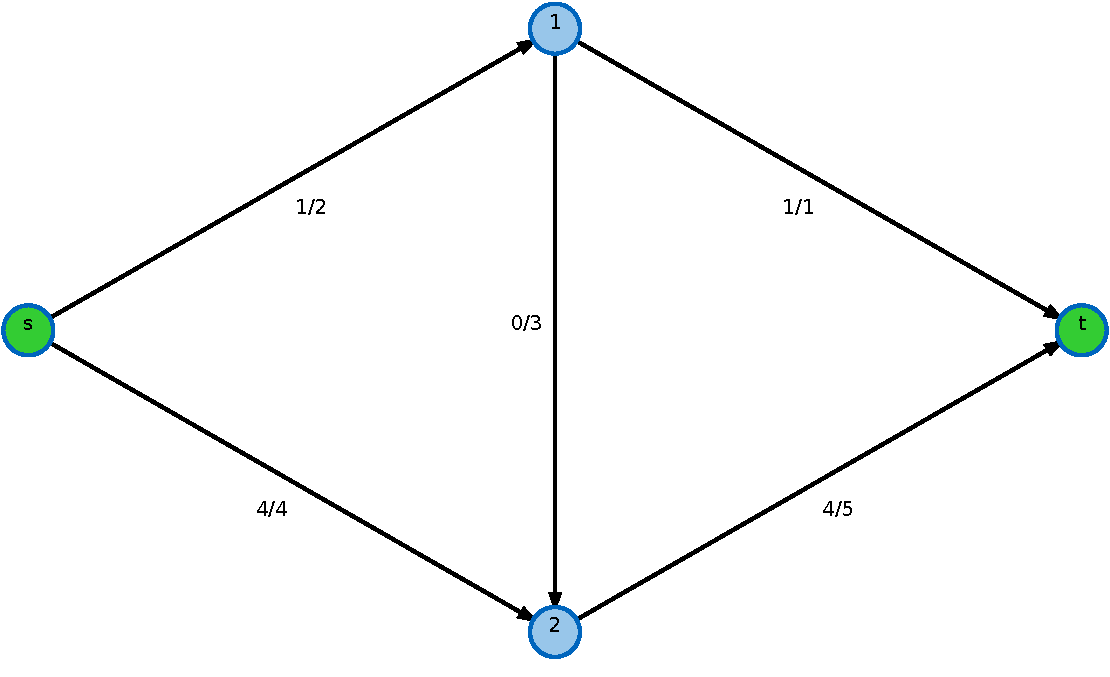
\includegraphics[width=0.8\textwidth]{img/network.pdf}
    \captionof{figure}{Ein Netzwerk mit Fluss.}
\end{minipage}
\begin{minipage}[t]{0.99\textwidth}
    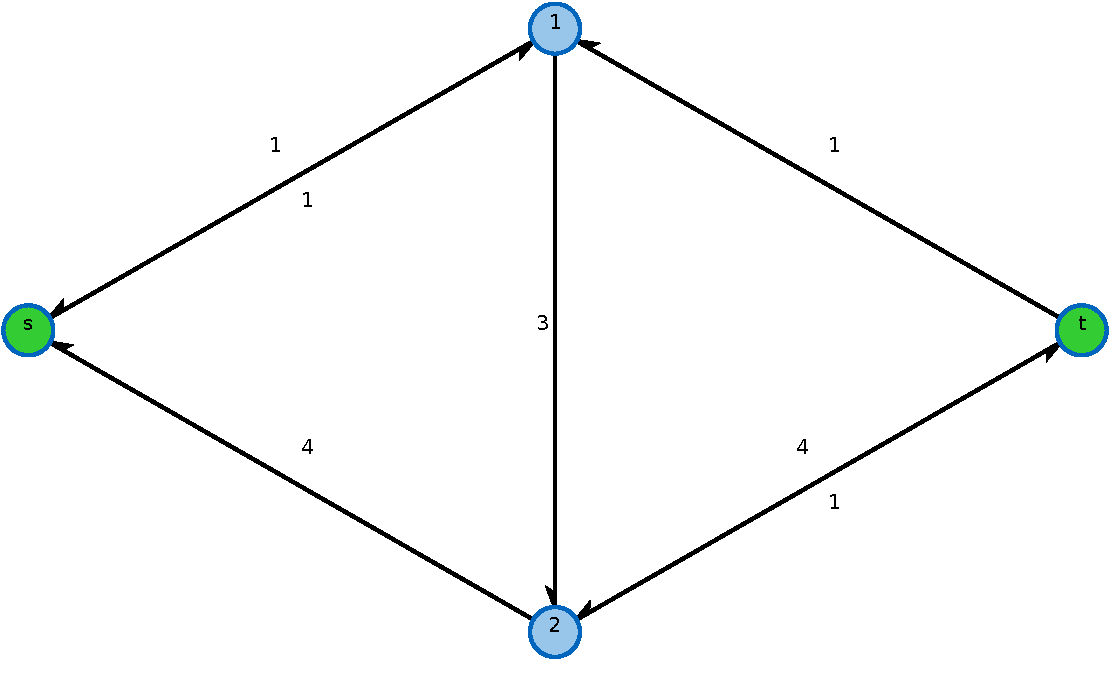
\includegraphics[width=0.8\textwidth]{img/network-residual.pdf}
    \captionof{figure}{Das zugehörige Residualnetzwerk.}
\end{minipage}

\section{Ford-Fulkerson Algorithmus}

Eine der naheliegenden Fragestellungen für ein gegebenes Netzwerk ist, wie viel Fluss gleichzeitig transportiert werden kann. Dies entspricht der Suche nach einem maximalen Fluss, das \emph{maximum flow problem}. Zur Berechnung maximaler Flüsse gibt es eine Reihe verschiedener Methoden, die sich in der Komplexität der Berechnung und Effizienz unterscheiden. Ein einfacher Algorithmus, der gleichzeitig Ausgangspunkt für eine Reihe an fortgeschritteneren Methoden bietet, ist der\emph{Ford-Fulkerson Algorithmus}. \cite{Ford-Fulkerson_algo}

Der Ford-Fulkerson Algorithmus berechnet den maximal möglichen Fluss, indem ausgehend von einem gültigen Fluss (dem Null-Fluss) wiederholt zusätzlicher Fluss durch das Netzwerk geschickt wird, ohne die Bedingungen zu verletzen. Sobald keine weiteren Änderungen mehr möglich sind ist der maximale Fluss gefunden.

Um eine gültige Änderung zu finden wird zunächst das Residualnetz des aktuellen Flusses konstruiert. In diesem wird dann ein Pfad gesucht, der Start- und Zielknoten verbindet. Entlang dieses \emph{augmentierenden Pfades} wird dann der Fluss um so viel erhöht, bis eine Kante saturiert und aus dem Residualnetz entfernt wird. Dies ist immer die Kante des Pfades mit der minimalen Residual-Kapazität. Diese Prozedur wird dann mit dem neuen Fluss wiederholt, bis kein Pfad mehr gefunden werden kann.

Die genaue Vorgehensweise für die Suche nach dem augmentierenden Pfad ist für den Ford-Fulkerson Algorithmus nicht exakt spezifiziert - sie hat allerdings starke Auswirkungen auf die Effizienz des Algorithmus. Naive Tiefensuche führt zu nichtpolynomieller Laufzeit $\mathcal{O}\left(|V|\cdot |E|\cdot u_{\max}\right)$, und auch das nur falls alle Kapazitäten ganzzahlig sind. Ein Breitensuche-Verfahren läuft dagegen schon in $\mathcal{O}(|V| \cdot |E|^2)$, diese spezielle Anwendung wird als \emph{Edmonds-Karp-Algorithmus} bezeichnet. \cite{Edmonds_karp} Eine weitere Verbesserung stellt mit einer Laufzeit von $\mathcal{O}(|V|^2 \cdot |E|)$ der \emph{Algorithmus von Dinic} dar, der nur kürzeste augmentierende Pfade verwendet. \cite{dinic70}\cite{Dinic}

\pagebreak
\begin{center}
\begin{minipage}[t]{0.65\textwidth}
    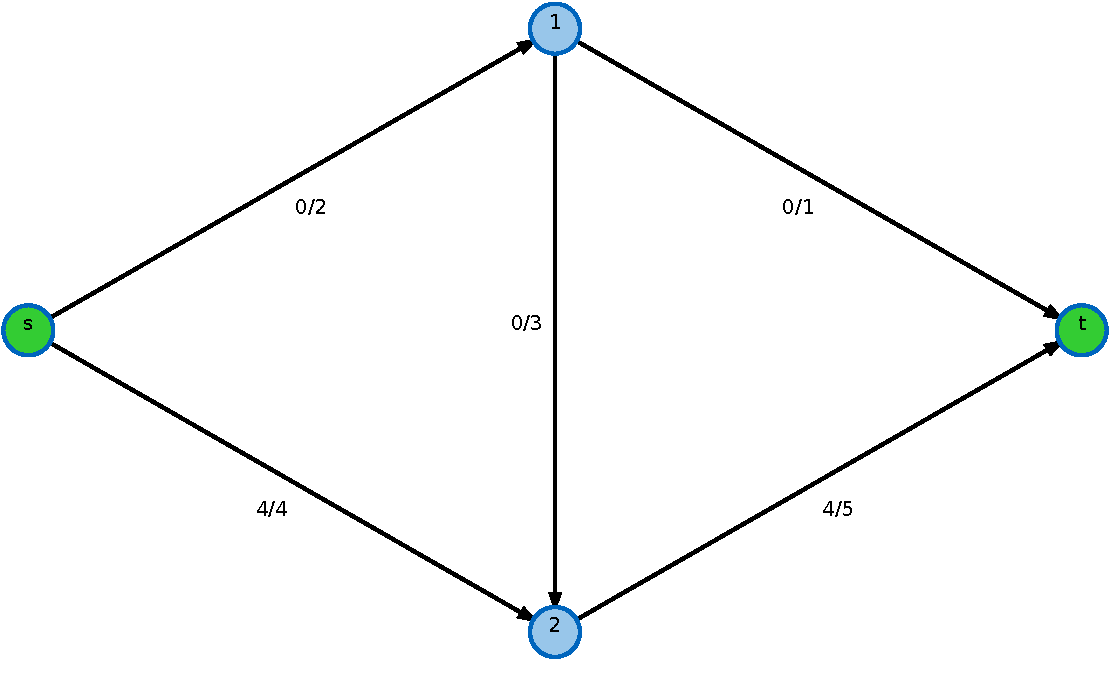
\includegraphics[width=\textwidth]{img/ford-fulkerson-1.pdf}
    \captionof{figure}{Ein initialer Fluss.}
\end{minipage}
\\
\begin{minipage}[t]{0.65\textwidth}
    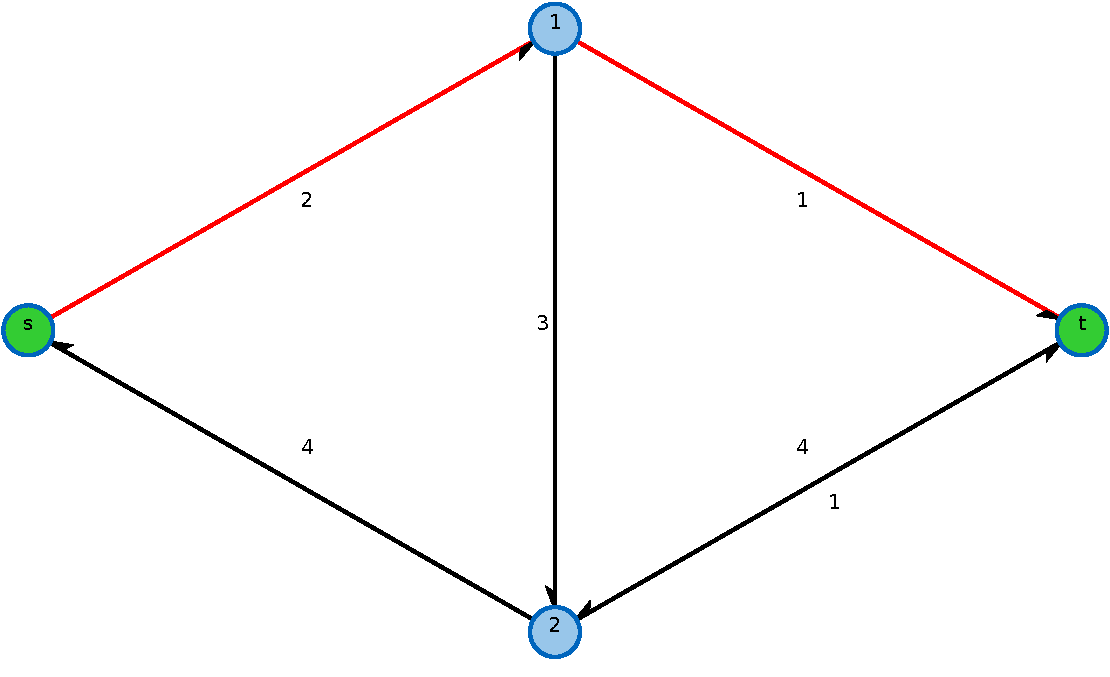
\includegraphics[width=\textwidth]{img/ford-fulkerson-2.pdf}
    \captionof{figure}{Ein augmentierender Pfad im Residualnetz.}
\end{minipage}
\\
\begin{minipage}[t]{0.65\textwidth}
    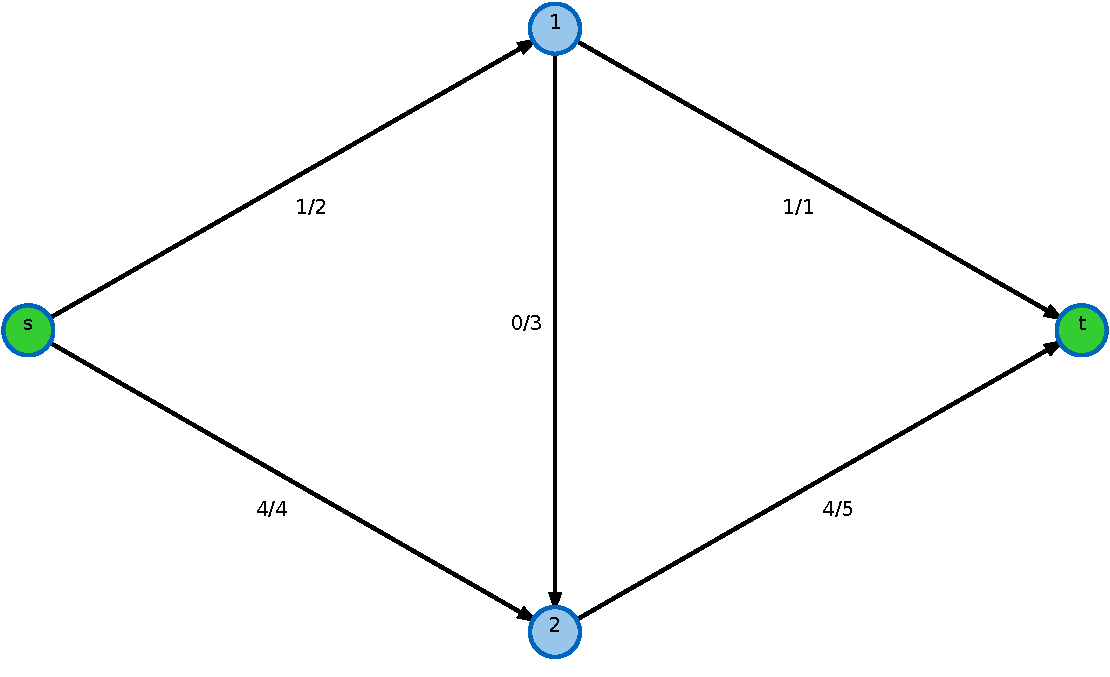
\includegraphics[width=\textwidth]{img/ford-fulkerson-3.pdf}
    \captionof{figure}{Der neue Fluss nach Modifikation.}
\end{minipage}
\end{center}

\section{Cycle Canceling Algorithmus}

Eine neue Klasse von Problemen stellt sich, sobald das Netzwerk zusätzlich mit einer Kostenfunktion auf den Kanten annotiert wird. Dies ist eine Funktion $c: E \rightarrow \mathbb{R}$ die jeder Kante zuordnet, wie teuer es ist, eine Einheit Fluss über die Kante zu transportieren. Für einen Fluss ergeben sich dann die Gesamtkosten als
\[C = \sum_{e \in E} c(e) \cdot f(e)\]

Es ergibt sich die Frage nach der günstigsten Möglichkeit, eine bestimme Menge an Fluss durch das Netzwerk zu leiten - das \emph{min-cost flow problem}. Eine übliche Variation ist zusätzlich den größtmöglichen Fluss (nach wie vor zu niedrigst möglichen Kosten) zu suchen, was man als \emph{min-cost max flow problem} bezeichnet.

Ein relativ einfacher Algorithmus zur Berechnung von Flüssen mit minimalen Kosten ist der \emph{Cycle Canceling Algorithmus}.\cite{cycle_canceling} Der Ansatz ist dem Ford-Fulkerson Algorithmus ähnlich, da auch hier eine eine vorläufige Lösung, ein gültiger Fluss der gesuchten Gesamtmenge, iterativ verbessert wird. Dazu werden Kreise im Residualnetz gesucht, die negative Gesamtkosten besitzen. Die Umleitung von Fluss entlang eines solchen Kreises verändert den Gesamtfluss nicht, senk allerdings die Kosten. Es kann so viel Fluss umgeleitet werden, bis die Kante des Kreises mit geringster Residualkapazität aus dem Residualnetz entfernt werden muss. Diese Ablauf kann wiederholt werden, bis keine negativen Kreise mehr im Residualnetz gefunden werden.

Zur Suche nach negativen Kreisen eignet sich der \emph{Bellman-Ford Algorithmus}, ausgeführt auf dem Residualgraphen mit den Kantenkosten als Gewichtungen und ausgehend vom Zielknoten. 

Der allgemeine Cycle Canceling Algorithmus führt zu einer nichtpolynomiellen Laufzeit in $\mathcal{O}\left(|V|\cdot |E|\cdot C_{max}\right)$, da jede Iteration eine Ausführung des Bellman-Ford Algorithmus mit Laufzeit $\mathcal{O}\left(|V|\cdot |E|\right)$ erfordert und die Kosten um mindestens $1$ verringert. Eine Abwandlung mit polynomieller Laufzeit stellt das \emph{Minimum Mean Cycle Canceling Verfahren} dar.\cite{min_mean_cycle_canceling}

\pagebreak
\begin{center}
\begin{minipage}[t]{0.60\textwidth}
    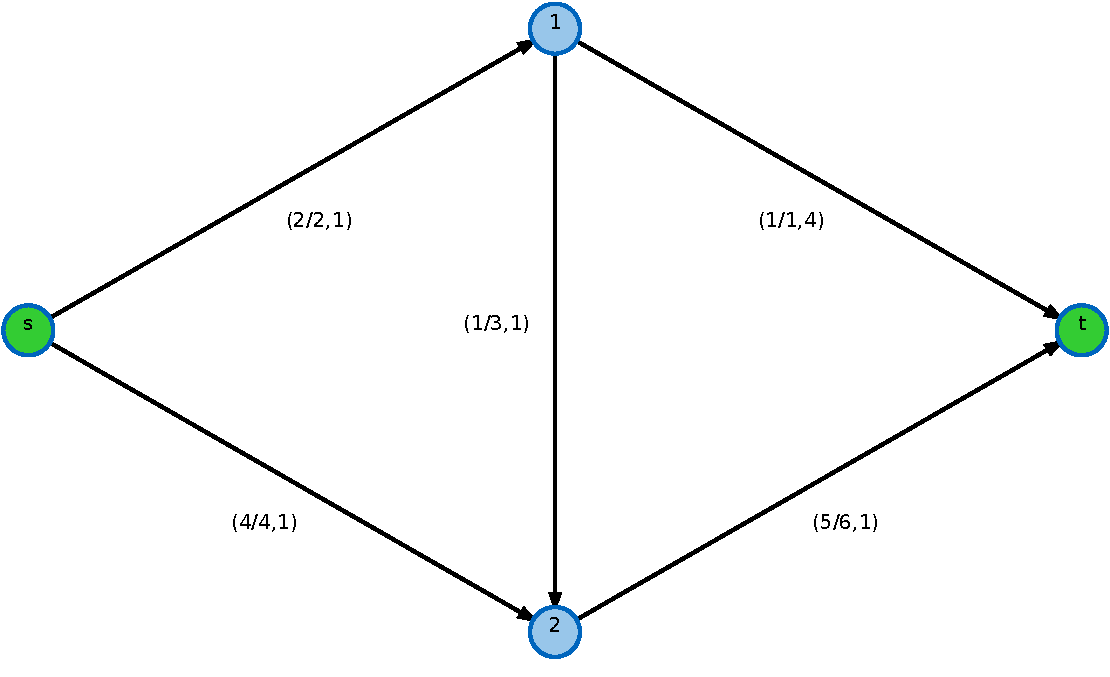
\includegraphics[width=\textwidth]{img/cycle-canceling-1.pdf}
    \captionof{figure}{Ein initialer maximaler Fluss.}
\end{minipage}
\\
\begin{minipage}[t]{0.60\textwidth}
    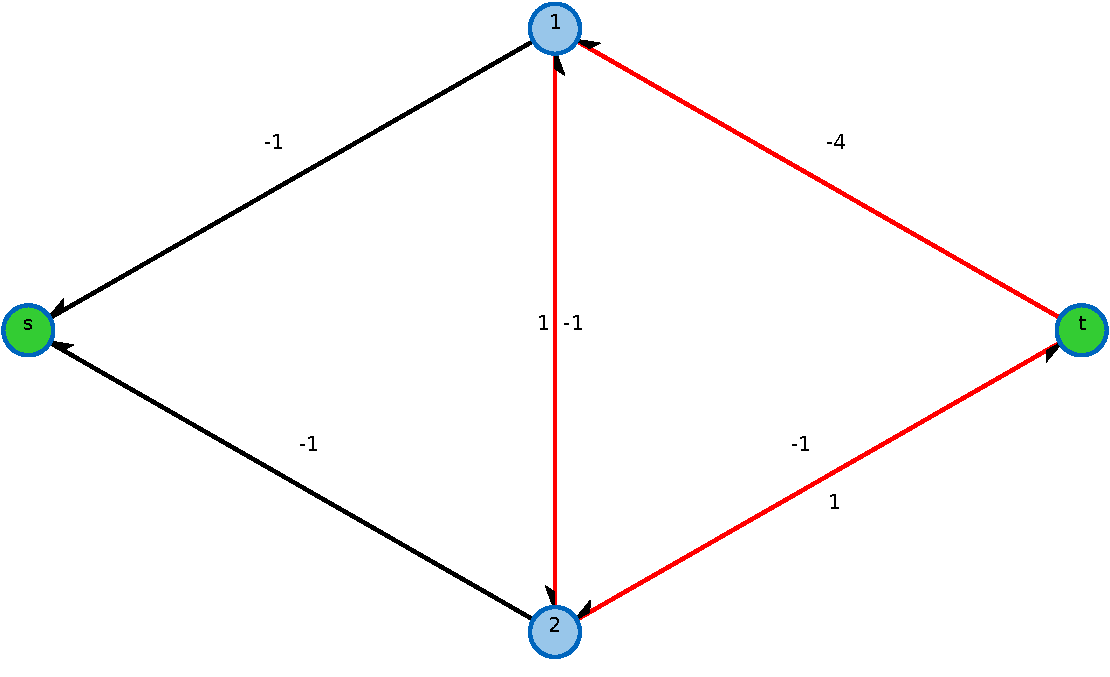
\includegraphics[width=\textwidth]{img/cycle-canceling-2.pdf}
    \captionof{figure}{Das Residualnetz enthält einen negativen Kreis.}
\end{minipage}
\\
\begin{minipage}[t]{0.60\textwidth}
    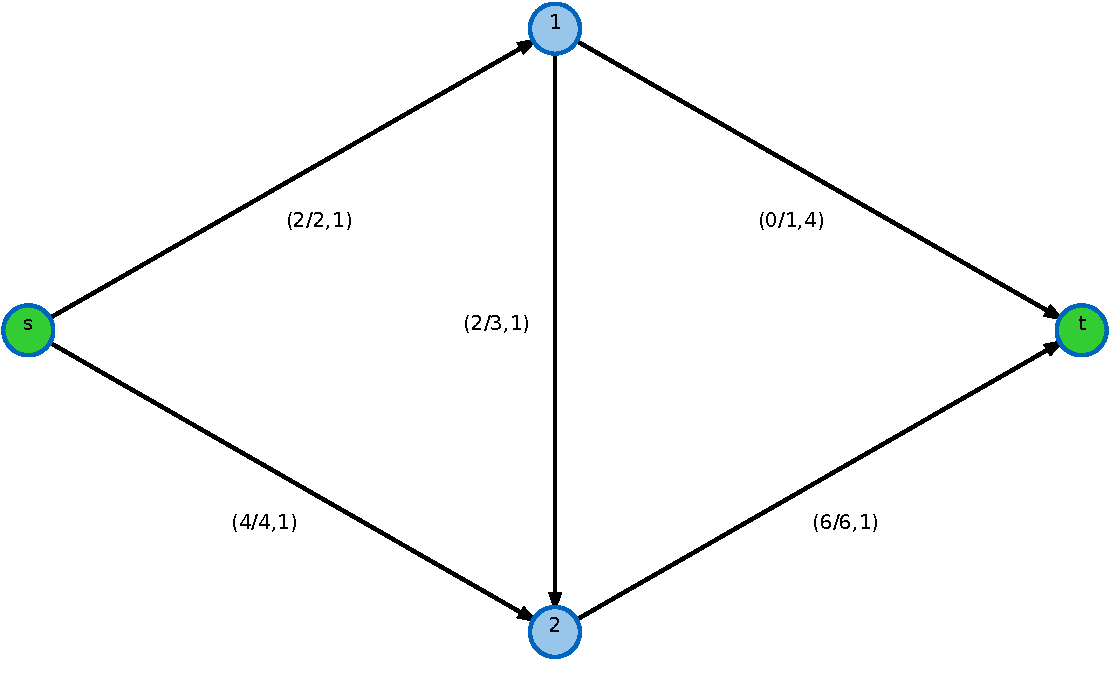
\includegraphics[width=\textwidth]{img/cycle-canceling-3.pdf}
    \captionof{figure}{Fluss nach Verschiebung entlang des negativen Kreises.}
\end{minipage}
\end{center}

\chapter{Aufbau der Webapplikationen}

\section{Framework für Graphalgorithmen}

Die Webapplikationen wurden in Analogie zu anderen, bereits bestehenden Applets für die Visualisierung verschiedener Graphalgorithmen konzeptioniert. Diese sind frei zugänglich auf der Webpräsenz des Lehrstuhls M5 für Mathematik an der TUM, erreichbar unter \href{https://www-m9.ma.tum.de/Allgemeines/GraphAlgorithmen}{https://www-m9.ma.tum.de/Allgemeines/GraphAlgorithmen}. 

Die bestehende Sammlung an Applets enthält bereits verschiedene andere Algorithmen der Graphentheorie, von Lösungsmethoden für des kürzeste Wege, Matchings, Spannbäume und mehr. Alle Anwendungen sind mit den gleichen Zielen entwickelt, die Algorithmen möglichst anschaulich und verständlich zu präsentieren, und verwenden das gleiche Seitenlayout. Auch die hier vorgestellten Applets zur Darstellung des Ford-Fulkerson Algorithmus und des Cycle Canceling Algorithmus stellen die Informationen in diesem bewährten Layout dar. Die Inhalte sind auf mehrere Tabs verteilt, die verschiedene Materialien bieten.

\paragraph{Tab: Einführung}

Die erste Einführung für den Benutzer gibt einen kurzen Überblick über die Problemstellung, die mithilfe des Algorithmus gelöst wird.
\begin{center}
\begin{minipage}[t]{0.80\textwidth}
    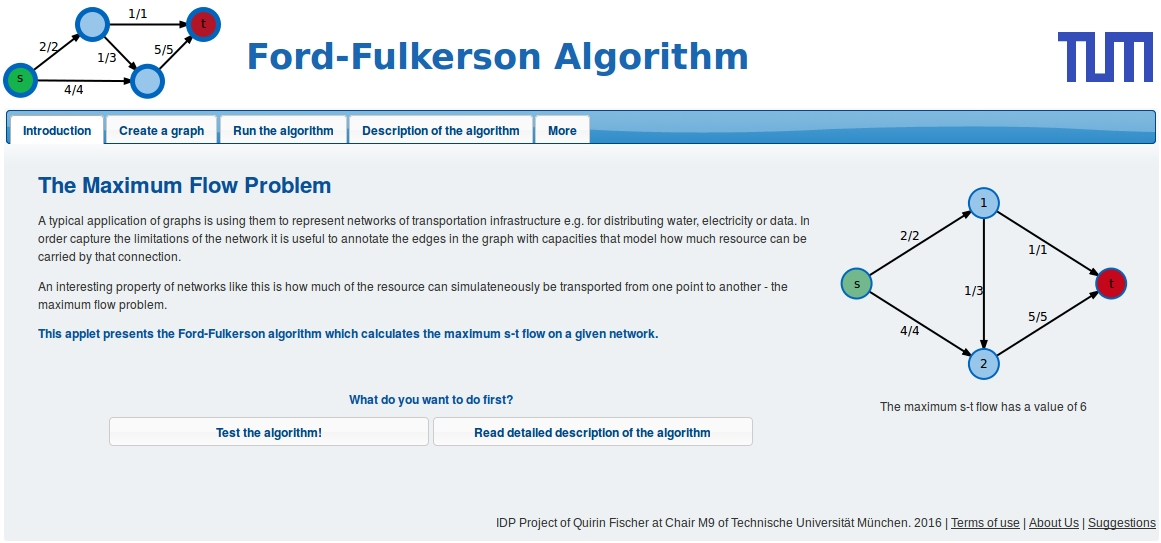
\includegraphics[width=\textwidth]{img/layout-1.jpg}
    \captionof{figure}{Der Einführungs-Tab.}
\end{minipage}
\end{center}
\vspace{1cm}

\paragraph{Tab: Grapherstellung} Ein Grapheditor, um die Instanz des Problems auszuwählen, auf der der Algorithmus ausgeführt werden soll. Der Editor bietet sowohl die Möglichkeit, vorgefertigte Beispiele zu laden, als auch diese zu verändern oder eigene Instanzen anzulegen. Knoten und Kanten des Graphen können einfach angelegt und gelöscht werden, und auf Klick ist auch die Modifikation zusätzlicher Eigenschaften wie Kantengewichte oder Kapazitäten möglich.

\begin{center}
\begin{minipage}[t]{0.60\textwidth}
    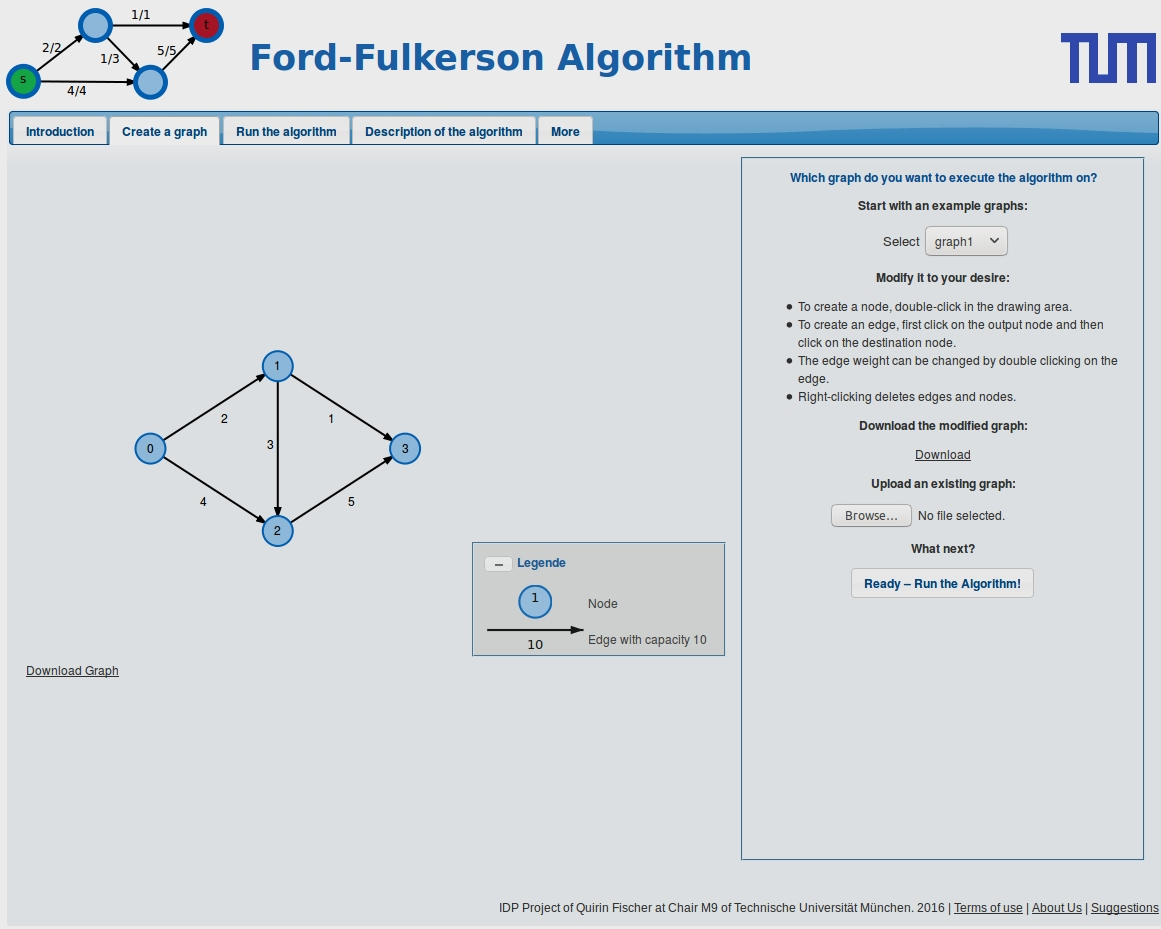
\includegraphics[width=\textwidth]{img/layout-2.jpg}
    \captionof{figure}{Der Tab des Grapheditors.}
\end{minipage}
\end{center}
\vspace{1cm}

\paragraph{Tab: Ausführung Algorithmus}

Der wichtigste Tab erlaubt die schrittweise Ausführung des Algorithmus und zeigt die internen Datenstrukturen. Einige Informationen werden grafisch in die Darstellung des Graphen integriert, indem beispielsweise Knoten oder Kanten farblich hervorgehoben werden. Eine seitliche Anzeige liefert wahlweise eine textuelle Beschreibung des aktuellen Arbeitsschrittes, die aktuelle Ausführungsposition in einer Pseudocode-Diagramm, oder die Werte von Variablen die der Algorithmus verwendet.

Die darzustellenden Daten unterscheiden sich zwischen den Algorithmen, so dass die Applikationen sich in diesem Tab am deutlichsten unterscheiden.

\begin{center}
\begin{minipage}[t]{0.60\textwidth}
    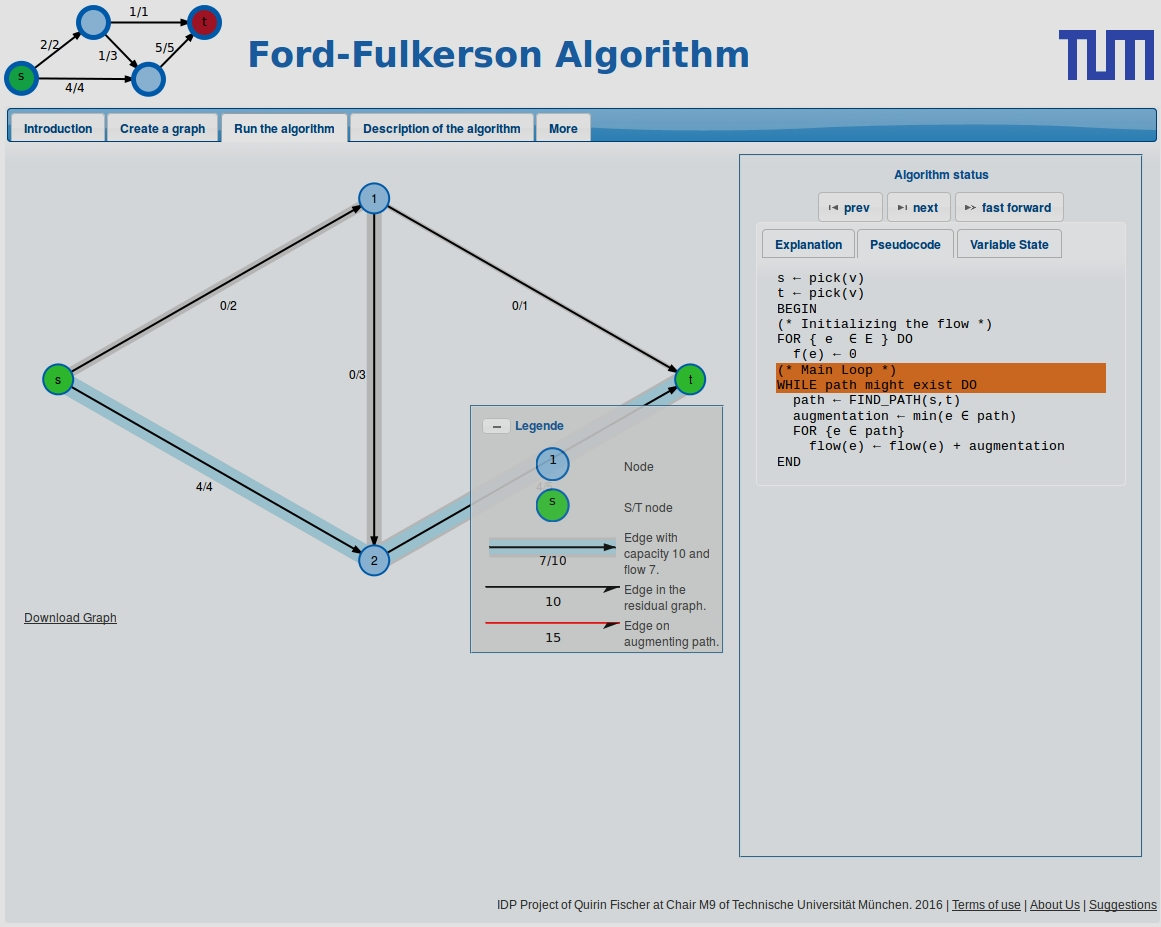
\includegraphics[width=\textwidth]{img/layout-3.jpg}
    \captionof{figure}{Der Algorithmus-Tab erlaubt schrittweise Ausführung und visualisiert den Status.}
\end{minipage}
\end{center}
\vspace{0.7cm}

\paragraph{Tab: Beschreibung Algorithmus}

Eine ausführlichere Beschreibung erläutert die Problemstellung und den genauen Ablauf des Algorithmus.

\begin{center}
\begin{minipage}[t]{0.60\textwidth}
    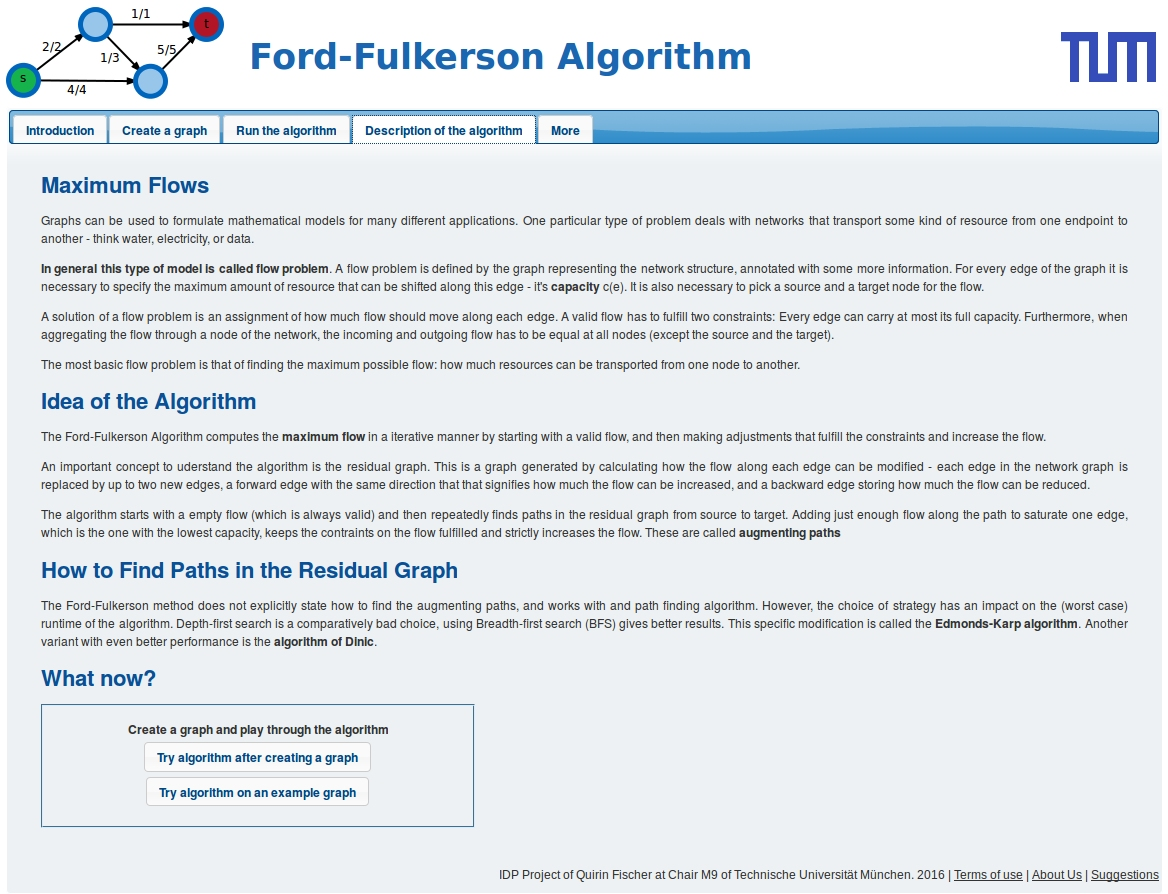
\includegraphics[width=\textwidth]{img/layout-4.jpg}
    \captionof{figure}{Eine längere Beschreibung des Algorithmus befindet sich im vierten Tab.}
\end{minipage}
\end{center}
\vspace{1cm}

\paragraph{Tab: Weitere Informationen}

Eine Sammlung nützlicher Informationen wie Beispielsweise einer Pseudocode-Darstellung des Algorithmus, Informationen zur Effizienz des Algorithmus, Hinweise auf abgewandelte Varianten oder eine Auswahl an Literatur und Referenzen.

\begin{center}
\begin{minipage}[t]{0.60\textwidth}
    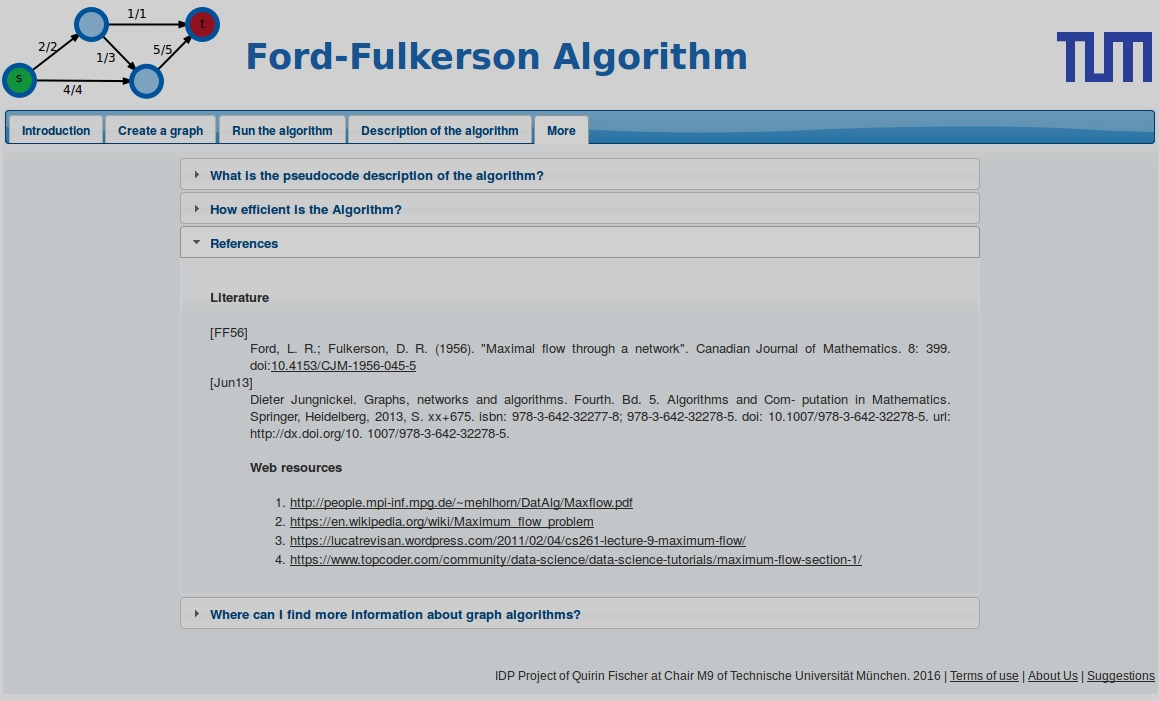
\includegraphics[width=\textwidth]{img/layout-5.jpg}
    \captionof{figure}{Der letzte Tab enthält weiteres Hintergrundmaterial.}
\end{minipage}
\end{center}


\section{Visualisierung des Ford-Fulkerson Algorithmus}

Während der Ausführung des Ford-Fulkerson Algorithmus verändert sind vor allem der Inhalt dreier Datenstrukturen: der aktuelle Fluss, das zugehörige Residualnetz, und sofern vorhanden der aktuelle augmentierende Pfad. Der Algorithmus alterniert Änderungen an diesen Daten - zunächst ist ein Fluss vorhanden, ausgehend von diesem wird das Residualnetz bestimmt, die Pfadsuche ergibt einen augmentierenden Pfad, woraufhin bei einem neuen Fluss begonnen wird. Die Visualisierung reflektiert diesen Ablauf und wechselt zwischen drei verschiedenen Ansichten.

In der ersten Ansicht wird ein Fluss visualisiert, indem die Kapazitäten und Flüsse der Kanten durch farbige Umrandung in verschiedenen Stärken dargestellt werden. Ein grauer Farbton zeigt freie Kapazität an, und eine helleres Blau zeigt vorhandenen Fluss. Diese Farbkodierung signalisiert klar, über welche Kanten der Fluss verläuft und wo sich freie Kapazität befindet.

Die zweite Ansicht zeigt das Residualnetzwerk des aktuellen Flusses. Die Richtungen der verfügbaren Kanten (oder der zugehörigen Rückkanten) werden durch Pfeilspitzen gekennzeichnet, mit Angabe der verfügbaren Kapazität auf der entsprechenden Seite der Kante. In der dritten Ansicht wird in diesem Netz der augmentierende Pfad farblich stark hervorgehoben, indem die Kanten des Pfades rot eingefärbt werden.

\begin{center}
\begin{minipage}[t]{0.58\textwidth}
    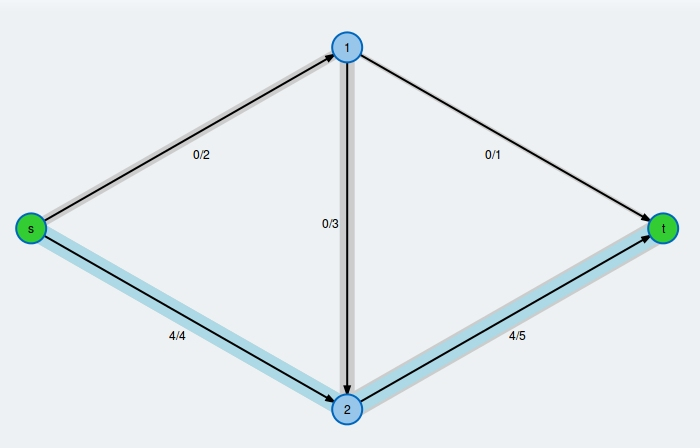
\includegraphics[width=\textwidth]{img/ford-fulkerson-1.jpg}
    \captionof{figure}{Flüsse und freie Kapazitäten werden farblich signalisiert.}
\end{minipage}
\end{center}


\begin{center}
\begin{minipage}[t]{0.58\textwidth}
    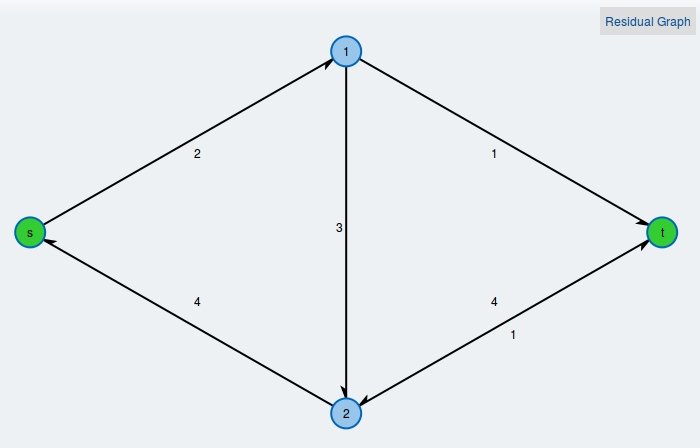
\includegraphics[width=\textwidth]{img/ford-fulkerson-2.jpg}
    \captionof{figure}{Das entsprechende Residualnetz.}
\end{minipage}
\end{center}


\begin{center}
\begin{minipage}[t]{0.58\textwidth}
    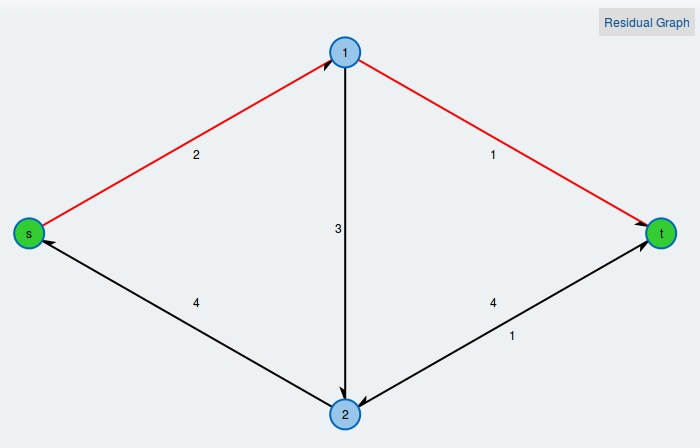
\includegraphics[width=\textwidth]{img/ford-fulkerson-3.jpg}
    \captionof{figure}{Der augmentierende Pfad wird rot gekennzeichnet.}
\end{minipage}
\end{center}


\section{Visualisierung des Cycle Canceling Algorithmus}

Auch der Cycle Canceling Algorithmus alterniert zwischen der Anzeige des aktuellen Flusses, des Residualnetzwerks, und des Residualnetzes mit hervorgehobenem negativen Kreis. Im Unterschied zum Ford-Fulkerson Algorithmus werden allerdings bei der Anzeige des Flusses zusätzlich die Kosten der Kanten angezeigt. Im Residualnetz sind die Kanten mit ihren Kosten beschriftet und nicht mit den Kapazitäten, da diese bei der Kreiserkennung verwendet werden. Die Visualisierung verwendet das gleiche Farbschema, negative Kreise werden also ebenfall in rot hervorgehoben.

\begin{center}
\begin{minipage}[t]{0.70\textwidth}
    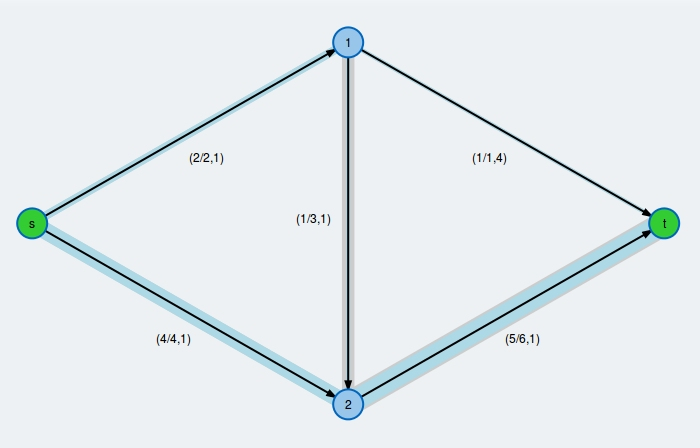
\includegraphics[width=\textwidth]{img/cycle-canceling-1.jpg}
    \captionof{figure}{Flüsse und freie Kapazitäten werden farblich signalisiert, mit zusätzlicher anzeige der Kosten.}
\end{minipage}
\end{center}


\begin{center}
\begin{minipage}[t]{0.70\textwidth}
    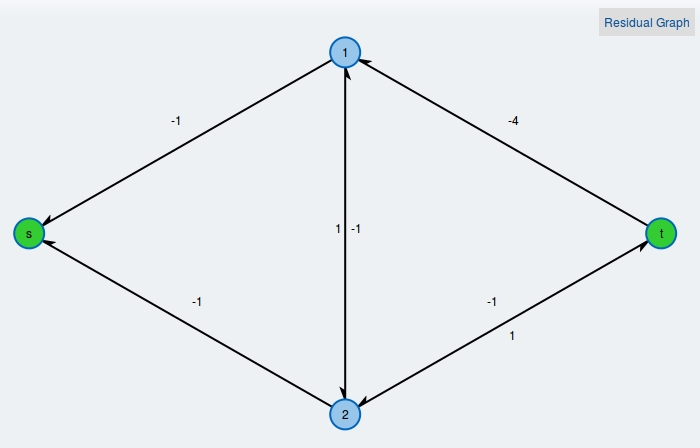
\includegraphics[width=\textwidth]{img/cycle-canceling-2.jpg}
    \captionof{figure}{Im Residualnetz sind die Kanten mit ihren Kosten beschriftet.}
\end{minipage}
\end{center}


\begin{center}
\begin{minipage}[t]{0.70\textwidth}
    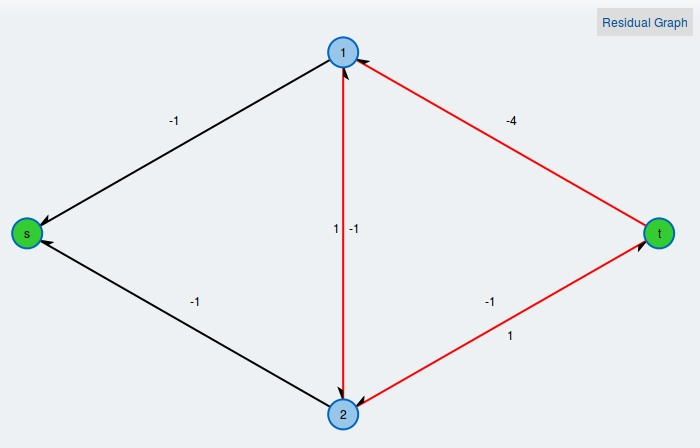
\includegraphics[width=\textwidth]{img/cycle-canceling-3.jpg}
    \captionof{figure}{Ein erkannter negativer Kreis wird in rot markiert.}
\end{minipage}
\end{center}

\chapter{Implementierung}

\section{Technische Konzepte}

Die technische Umsetzung der Webapplikationen erfolgt ausgehend von der bestehenden Code-Struktur ähnlicher Andwendungen für andere Algorithmen. Das Framework umfasst die generelle Seitenstruktur, die Tabverwaltung, ein Grapheditor und eine Grundgerüst für die schrittweise Ausführung eines Algorithmus. Implementiert als interaktive Website besteht die Codebasis aus einer Mischung von HTML, CSS und Javascript. 

Im Folgenden werden zunächst die verwendeten Technologien und verwendete Muster vorgestellt. Da der bestehende Quellcode eine relative enge Vermengung von Framework-code mit Algorithmus-spezifischen Teilen erforderte, so dass im Anschluss einige funktionale Einheiten des Quellcodes vorgestellt werden.

\paragraph{HTML5 / CSS}
Das HTML Dokument stellt das statische Gerüst der Website dar. Es bindet die verschiedenen Skripte zur Kontrolle der interaktiven Elemente ein, enthält die statischen Textinhalte, und definiert Platzhalter für die Anzeige dynamischer Elemente. Der HTML Code befindet sich in den Dateien \texttt{max-flow/index\_en.html} und \texttt{min-cost/index\_en.html}. Einstellungen für die Darstellung verschiedener Webseiten-Elemente befinden sich in den CSS Dateien in \texttt{library/css} und \texttt{library-d3-svg/css}.

\paragraph{Javascript}
Die Interaktiven Elemente des Graph-Editors und des Algorithmus-Tabs sind mittels Javascript implementiert. Dies umfasst die folgenden Bereiche:

\begin{description}
    \item [Verwaltung der dynamischen Tabs] Bei Öffnung und Schließen der Tabs wird die Anzeige initialisiert, und optional wird der Benutzer drauf hingewiesen, dass bei Verlassen des Tabs der Zustand zurückgesetzt wird.
    \item [Entgegennahme von Benutzereingaben] Für die Bearbeitung des Graphen und während der Auswahl von Start/Zielknoten müssen Einagbe-Events entgegengenommen werden.
    \item [Ausführung von Algorithmus-Schritten] Berechnung der einzelnen Schritte des Algorithmus.
    \item [Graphdarstellung] Für die Visualisierung muss der angezeigte Graph an die internen Daten angepasst werden.
\end{description}

\paragraph{SVG}

Die Darstellung des Graphen geschieht als Vektorgrafik. Die Javascript-Routinen modifizieren dafür zwei \texttt{<svg>} Elemente die als Anzeige für Editor und Algorithmus dienen, fügen die nötigen geometrischen Primitiven ein und setzen deren Rendering-Einstellungen. So wird beispielsweise für jeden Knoten des Graphen ein farbiger Kreis und ein Textelement mit der Beschriftung erzeugt; falls der Knoten als Start oder Ziel ausgewählt wird, so wird die Füllfarbe des Kreises geändert.

\paragraph{D3.js}

Für die dynamische Anpassung des Dokuments ist es nötig, das sogenannte \emph{Document Object Model(DOM)} zu ändern. Diese Synchronisierung von komplexeren internen Daten (dem Graphen) mit einer Menge an Elementen des Dokuments erfolgt mithilfe der Javascript-Bibliothek \emph{D3.js}\cite{d3js}.


\section{Code-Komponenten und deren Interaktion}

\subsection{Struktur der statischen Seite}

Die verschiedenen Tabs sind innerhalb des Hauptelements mit der ID \texttt{tabs} definiert. Dieses befindet sich in \texttt{max-flow/index\_en.html} (Z.145) bzw. \texttt{min-cost/index\_en.html} (Z.144). Die Struktur sieht wie folgt aus:

\begin{lstlisting}[caption=Tabstruktur,language=HTML]
<div id="tabs">
  <ul>
    <li><a href="#tab_te"><span>Introduction</span></a></li>
    <li><a href="#tab_tg"><span>Create a graph</span></a></li>
    ...
  </ul>
  <div id="tab_te"> 
    (Introduction content: ...)
  </div>
  <div id="tab_tg"> ... </div>
  ...
</div>
\end{lstlisting}

Innerhalb des Tab-Sektionen befinden sich die einzelnen Inhalte und Texte. Die dynamischen Tabs enthalten je einen Platzhalter für die erzeugten Vektorgraphiken, in \texttt{max-flow/index\_en.html} (Z.184, Z.261) bzw. \texttt{min-cost/index\_en.html} (Z.191, Z.262). Für dynamische Tabs definiert das Framework noch einige Init/Exit Routinen, diese befinden sich u.A. in \texttt{library-d3-svg/js/Tab.js} und \texttt{max-flow/js/siteLayout.js} bzw. \texttt{min-cost/js/siteLayout.js}.


\subsection{Verwaltung der Graphdaten}

Die Graphdaten werden mithilfe des Modells definiert in \texttt{library-d3-svg/js/Graph.js} verwaltet. Das Datenmodell sorgt dafür, dass die Struktur sowohl für den Editor als auch den Algorithmus zugänglich ist. Knoten und Kanten sind per Index auswählbar und enthalten jeweils Adjazenzlisten. Jedes Element des Graphen kann eine Menge an Ressourcen (z.B. Kapazitäten) und Statusinformationen (z.B. Vorgänger-Informationen während der Pfadsuche) mitführen. Der Grapheditor ist in \texttt{library-d3-svg/js/GraphEditor.js} und \texttt{library-d3-svg/js/GraphEditorTab.js} implementiert.
.

\subsection{Schrittweise Ausführung des Algorithmus}

Die Ausführung des Algorithmus mit den Möglichkeiten der schrittweisen Navigation erfordert eine klare Verwaltung der Zustandsänderungen im Algorithmus.  Dies erfolgt mit der folgenden Struktur:

Der aktuelle Zustand ist in der Variable \texttt{state} \texttt{max-flow/js/FordFulkersonAlgorithm.js} (Z.326) bzw. \texttt{min-cost/js/CycleCancelingAlgorithm.js} (Z.305) gespeichert, mit zusätzlicher Statusinformation eingebettet in den Graphen. Beim Durchlaufen des Algorithmus werden diese Statusinformationen in eine Historie kopiert, um eine Rückwärtsnavigation zu erlauben.

\begin{lstlisting}[caption=Historie der Berechnungsschritte,language=Javascript]
this.addReplayStep = function(){
  replayHistory.push({
    "graphState": Graph.instance.getState(),
    "state": JSON.stringify(state),
    ...
  });
};

this.previousStepChoice = function() {
  var oldState = replayHistory.pop();
  Graph.instance.setState(oldState.graphState);
  state = JSON.parse(oldState.state);
  ...
  this.update();
};
\end{lstlisting}

\pagebreak

Die Ausführungslogik des Algorithmus muss in einzelnen Teilfunktionen gegliedert werden, die je nach aktuellem Berechnungsfortschritt (gespeichert in \texttt{state.current\_step}) die Berechnungen auf den Status anwendet.

\begin{lstlisting}[caption=Schrittweise Ausführung des Algorithmus, language=Javascript]
this.nextStepChoice = function(d) {
  // Speichere aktuellen Schritt im Stack
  this.addReplayStep();
  switch (state.current_step) {
    case STEP_SELECTSOURCE:
      this.selectSource(d);
      break; 
    ...   
    case STEP_FINDNEGATIVECYCLE:
      findNegativeCycle();
      break;
    case STEP_ADJUSTCYCLE:
      adjustCycle();
      break;
    ...
  }
  this.update();
};

function adjustCycle() {
  for(var i = 0; i < state.cycle.length; ++i)
  {
    var edge = Graph.instance.edges.get(state.cycle[i]["edge"]);

    edge.state.flow += state.cycle_min_flow * state.cycle[i]["direction"];
  }
  state.cycle_min_flow = 0;
  state.cycle = [];
  state.show_residual_graph = false;
  state.current_step = STEP_MAINLOOP; 
}
\end{lstlisting}

\subsection{Darstellung der Graph-Visualisierung}

Die Generierung der Vektorgrafik zur Anzeige des Graphen erfolgt größtenteils in \texttt{library-d3-svg/js/GraphDrawer.js}. Zusätzlich können die einzelnen Algorithmen noch Modifikationen durchführen, um zusätzliche Informationen anzuzeigen. So werden beispielsweise die Beschriftung und Farbe von Start- und Zielknoten verändert, oder die Kanten verschieden gestaltet um Fluss zu signalisieren.

\begin{lstlisting}[caption=Algorithmus-spezifische Visualisierung, language=Javascript]
this.onNodesUpdated = function(selection) {
  selection
    .selectAll("circle")
      .style("fill", function(d) {
        if (d.id == state.sourceId)
          return const_Colors.StartNodeColor; //green
        else if (d.id == state.targetId)
          return const_Colors.StartNodeColor; //green
        else
          return global_NodeLayout['fillStyle'];
      });
}

this.onEdgesEntered = function(selection) {
  selection.append("line")
    .attr("class", "cap")
    .style("stroke-width",
        function(d) {
          return algo.flowWidth(d.resources[0]);
        });

  selection.append("line")
    .attr("class", "flow");
}
  
this.onEdgesUpdated = function(selection) {
  selection.selectAll("line.flow")
    .style("stroke-width",
      function(d) {
      return algo.flowWidth(Graph.instance.edges.get(d.id).state.flow); });      
  ...
}
\end{lstlisting}

\subsection{Synchronisierung von Anzeige und Berechnungszustand}

Um den aktuellen Status des Algorithmus sichtbar zu machen, befinden sich innerhalb des Algorithmus-Tabs drei weitere Tabs um eine Beschreibung des aktuellen Schritts, den aktuellen Schritt in Pseudocode, und die aktuellen Variablenwerte anzuzeigen. Die Beschreibungen und Pseudocode-Informationen sind im HTML Dokument gelistet und werden mithilfe von D3.js ein/ausgeblendet oder farbig markiert. Für die Variablenwerte wurden Platzhalter im HTML platziert, in die Werte eingetragen werden.


\begin{lstlisting}[caption=Tabs zur Anzeige des aktuellen Status des Algorithmus, language=HTML]
<div id="ta_div_statusTabs">
  <ul>
    <li><a href="#ta_div_statusErklaerung">Explanation</a></li>
    <li><a href="#ta_div_statusPseudocode">Pseudocode</a></li>
    <li><a href="#ta_div_variables">Variable State</a></li>
  </ul>
  <div id="ta_div_statusErklaerung">
    <div id="explanation-select-source">
      <h3>First choose a source node</h3>
      <p>Click on a node to select it as the source/starting node s</p>
    </div>
    <div id="explanation-select-target">
      <h3>Then choose a target node</h3>
      <p>Click on a node to select it as the target/sink node t</p>
    </div>
    ...
   </div>
  <div class="PseudocodeWrapper" id="ta_div_statusPseudocode"> ... </div>
  <div id="ta_div_statusVariables">
    <h3>Variable State</h3>
    <table class="algoInformationen">
      <tr>
        <th class="algoInfoTH"><span>cycle</span></th>
        <th class="algoInfoTH"><span>adjustment</span></th>
      </tr>
      <tr>
        <td id="variable-value-cycle" class="algoInfoTD">-</td>
        <td id="variable-value-adjustment" class="algoInfoTD">-</td>
      </tr>
    </table>
  </div>
</div>
\end{lstlisting}


\begin{lstlisting}[caption=Anzeige des aktuellen Status, language=Javascript]
this.updateDescriptionAndPseudocode = function() {
  var sel = d3.select("#ta_div_statusPseudocode").selectAll("div");
  sel.classed("marked", function(a, pInDivCounter, divCounter) {
    return d3.select(this).attr("id") === "pseudocode-"+state.current_step;
  });
  var sel = d3.select("#ta_div_statusErklaerung").selectAll("div");
  sel.style("display", function(a, divCounter) {
    return (d3.select(this).attr("id") === "explanation-"+state.current_step) ? "block" : "none";
  });
  ...
};

this.updateVariables = function() {
  ... 
  var path_string = "["+path_edge_strings.join(",")+"]";
  d3.select("#variable-value-path").text(path_string);
  d3.select("#variable-value-augmentation").text(state.augmentation);
}
\end{lstlisting}
\addcontentsline{toc}{chapter}{Fazit}
\chapter*{Fazit}
% appendices (if appropriate)
\appendix
% all appendices behind backmatter will go without numbers
\backmatter

%List of Figures
\listoffigures

%List of Code Listings
\lstlistoflistings 

\vspace*{1.5cm}

%List of Tables
%\listoftables


%List of algorithms
% only in conjunction with algorithm2e
%\phantomsection% for hyperref
%\addcontentsline{toc}{chapter}{Algorithmenverzeichnis}%
%\markboth{Algorithmenverzeichnis}{Algorithmenverzeichnis}
%\listofalgorithms


%Algorithmenverzeichnis
% nur in Verbindung mit algorithm2e
%\phantomsection% fuer hyperref
%\addcontentsline{toc}{chapter}{Algorithmenverzeichnis}%
%\markboth{Algorithmenverzeichnis}{Algorithmenverzeichnis}
%\listofalgorithms

% Index
% Add index to table of contents
%\addcontentsline{toc}{chapter}{Index}
%\printindex

% Bibliography
\printbibliography[heading=bibintoc]

%In the final version, this should be empty and needn't be commented out. Someone who works sloppily should at least remember to comment out the fixme list, so that unfinished places are
%not so obvious for the examiners.
%\listoffixmes
%
\end{document}
% ==============================================================================
% End of document
% ==============================================================================